% !TeX root = ../main.tex

\chapter{多租户性能隔离的闪存资源池化系统设计}
\label{chap:design}

本章介绍本研究提出的多租户性能隔离的闪存资源池化系统设计。
\autoref{sec:design-overview}是对该系统各组件的功能和每一租户获取、访问资源的流程概述。
为了提供没有读写干扰的SSD访问尾延迟,\autoref{sec:design-array}介绍了本系统通过将SSD的访问时间窗口划分为独立的纯读和纯写窗口,避免

\section{系统总述}
\label{sec:design-overview}

如\autoref{fig:design-overview}所示,本系统主要由控制器、客户端和存储单元组成。
其中,控制器负责管理存储单元,并根据租户的需求用尽可能经济的方式为其分配存储空间。
为了避免存储空间的碎片化,控制器以\textit{块}为单位管理存储空间,例如10GB为一个块。
客户端位于租户的虚拟机上,它负责与控制器沟通,并代替租户进行存储资源访问。
存储单元可能是一块SSD或多块SSD组成的存储阵列(~\autoref{sec:design-array}),不同的存储单元可以提供不同的SLA保证,也有不同的开销。
例如,一个存储单元可能用3块SSD的冗余提供99\%分位数的尾延迟保证,而另一个存储单元可能仅能提供90\%的保证,但只需要花费一块SSD。

\begin{figure}[h]
  \centering
  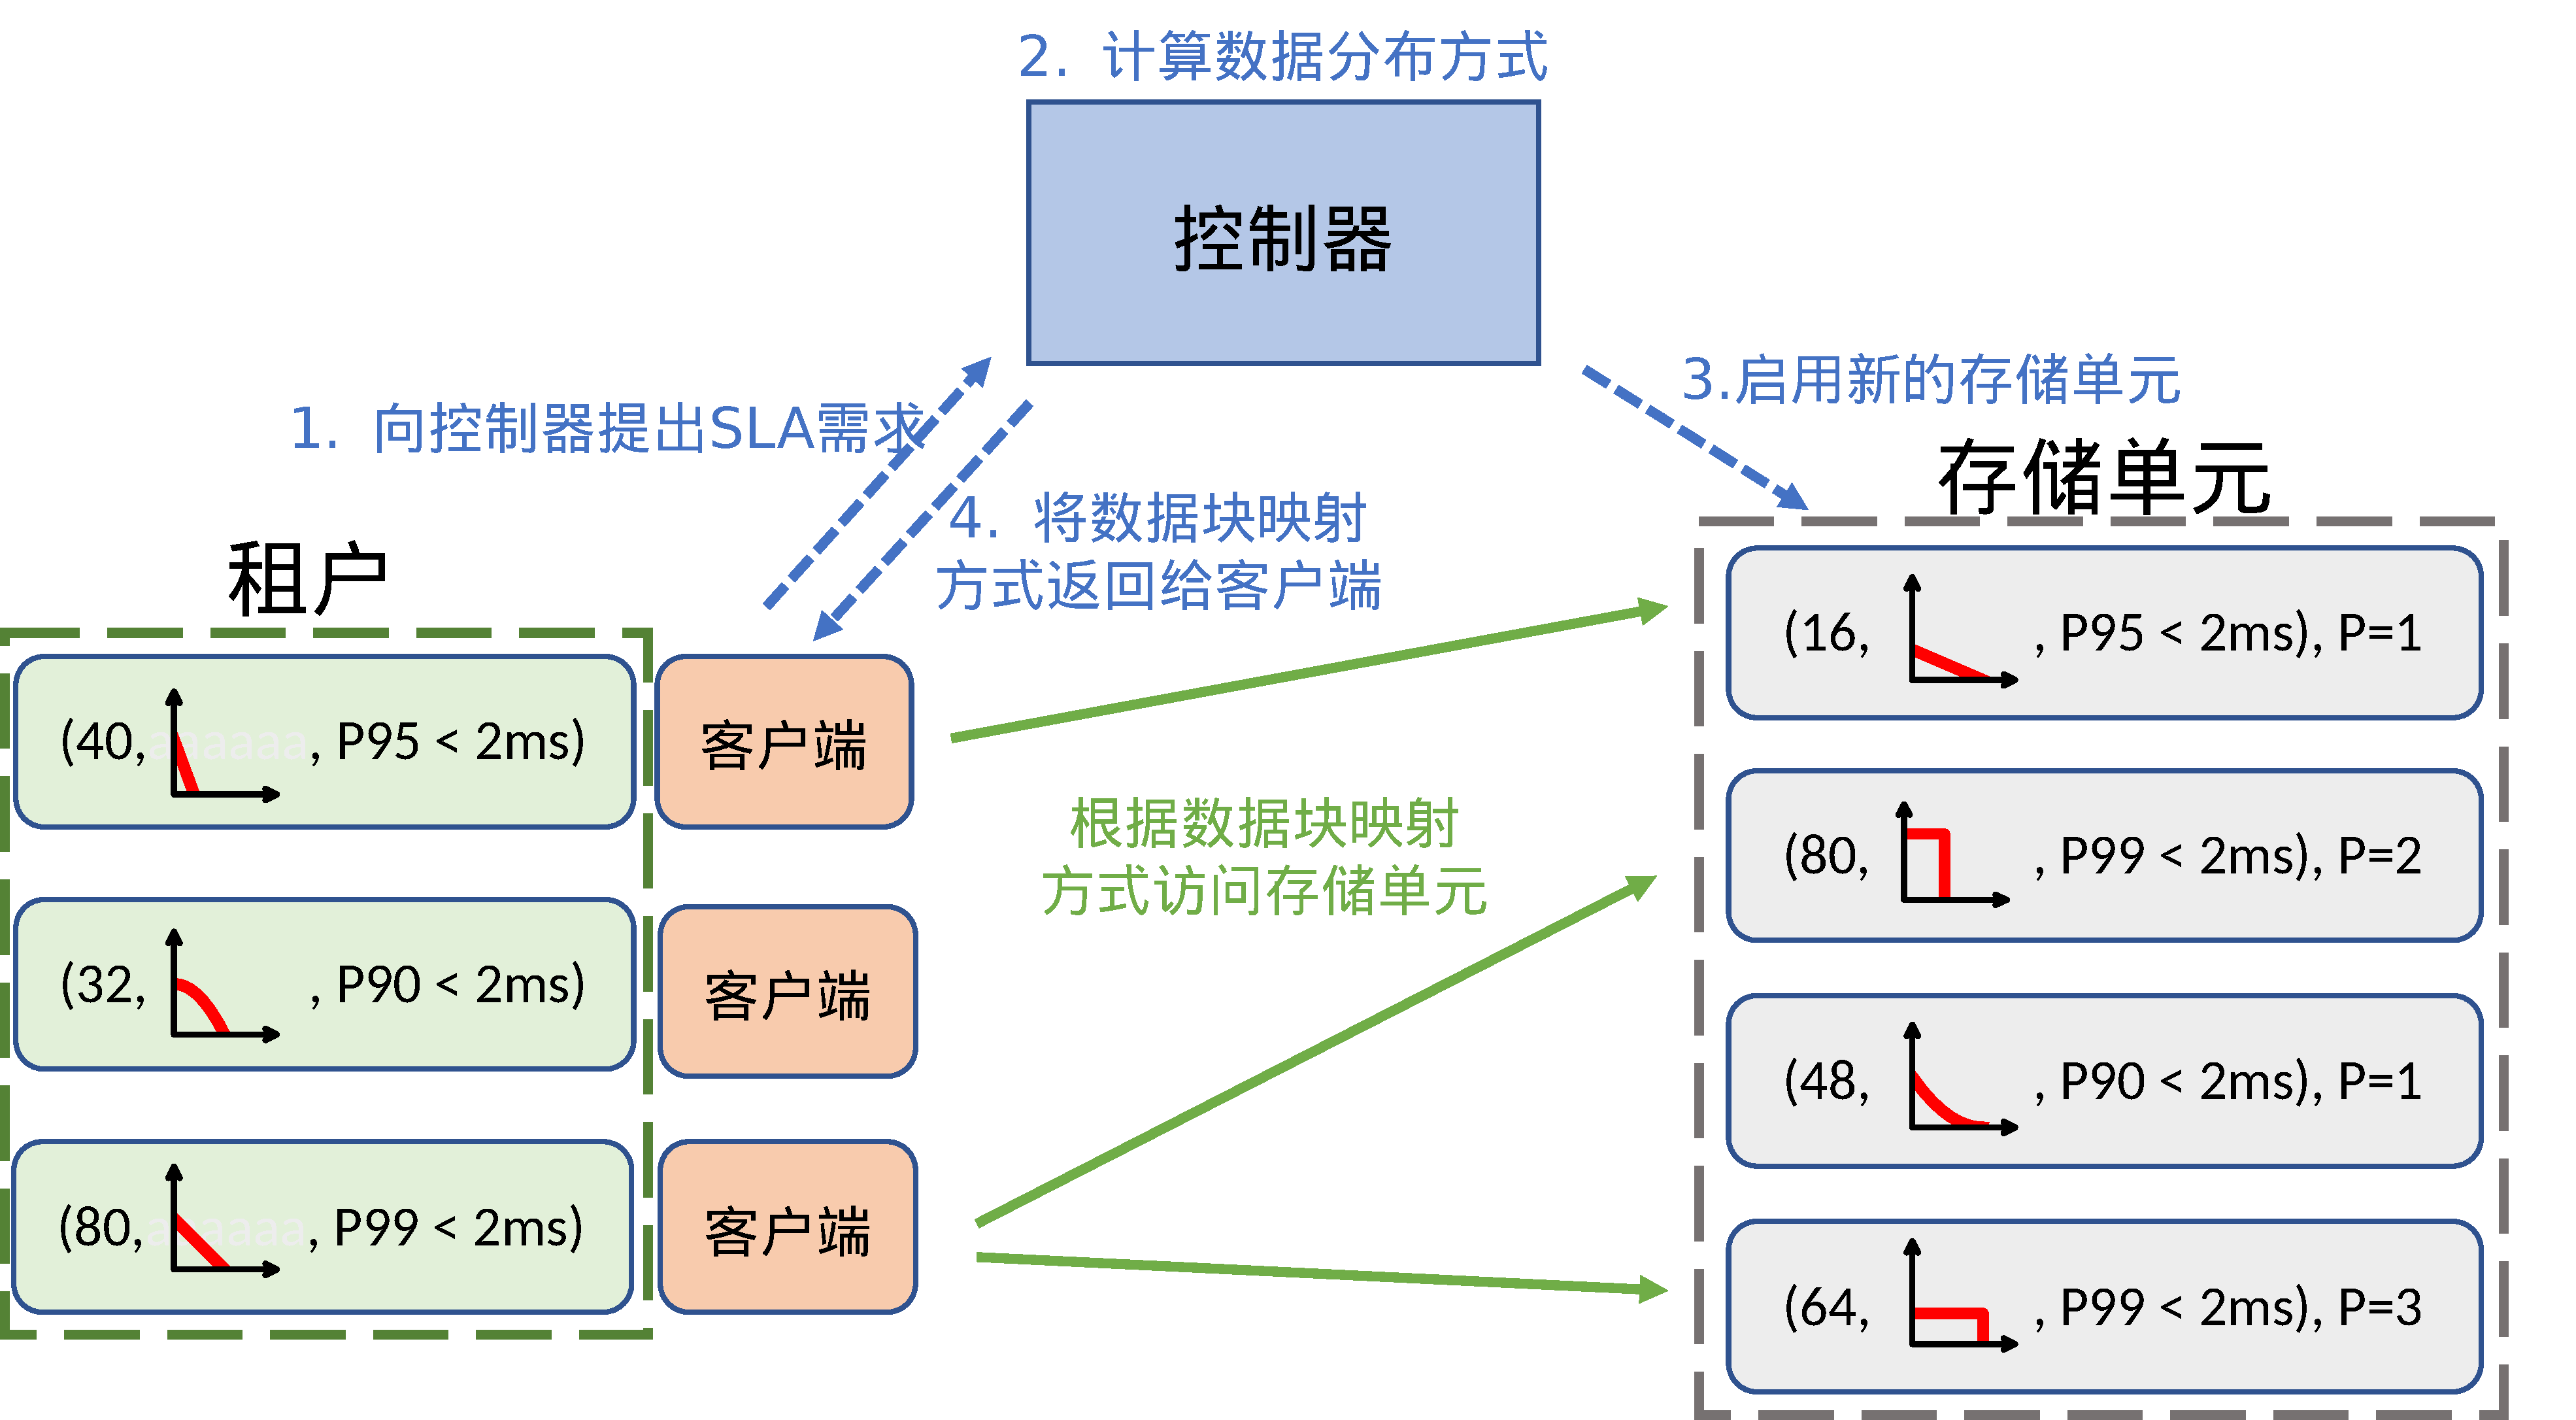
\includegraphics[width=0.8\textwidth]{thesis-design.pdf}
  \caption{
      本系统的总体概述。
      图中蓝色虚线标示的是新租户进入本系统时的控制路径,
      绿色实线标示的是系统中的租户访问存储单元时的数据路径。
      }
  \label{fig:design-overview}
\end{figure}

在本系统中,每个租户的资源需求和每个存储单元能提供的服务能力均以$(C, S, T)$这一三元组定义。
其中,$C$表示存储空间(Capacity),例如40个块;
$S$表示SLA曲线(SLA Curve);
$T$表示尾延迟要求(Tail latency),例如延迟的99\%分位数小于2ms($P99 < 2ms$)。 
由于存储单元的异构性,每个存储单元还有自身的开销$P$。

本系统的控制路径由\autoref{fig:design-overview}中的蓝色虚线表示。
当一个用户加入系统时,他首先通过客户端将自己的资源需求以以上三元组的形式发送给控制器。
控制器以块为单位管理用户的存储需求。
由于每个用户的各个块之间是条带化的\cite{patterson1988case},因此SLA曲线也可以平均分配到每个块上。
根据\autoref{sec:design-allocation}中提出的启发式数据分布算法,控制器优先将尽可能多的块放于已启用的存储单元上。
若已启用的存储单元不足以容纳用户的资源需求,则根据存储单元的开销$P$选择最经济的方式存放剩余的存储需求。
此时若有需要,控制器还需要负责建立新的存储单元(\autoref{sec:design-array})。
在控制器确定该用户的数据分布后,他将该租户的存储空间中每个块与对应的存储单元及存储单元中该块的起始地址的映射发送给租户服务器上的客户端。

\autoref{fig:design-overview}中的绿色实线表示的是本系统的数据路径。
当租户需要访问其所拥有的存储空间时,客户端根据该映射选择合适的存储单元,并将租户存储空间内的逻辑地址转换为存储单元的逻辑地址,从而代替租户访问存储单元。
客户端根据租户的SLA曲线对租户的读写速率进行限制,从而保证租户得到自身的SLA保证。
该客户端可以实现在软件的块设备层~\cite{linuxblock},也可以在智能网卡通过硬件实现~\cite{bluefield}。

\section{无读写干扰的SSD阵列}
\label{sec:design-array}

云存储系统的某些租户可能具有苛刻的尾延迟要求。
然而,如\autoref{fig:bg-wr-interfere}所示,SSD上程度很小的读写干扰就可能使其尾延迟难以达到租户的要求。
因此,本节提出无读写干扰的SSD阵列,它可以在读写吞吐都很大的情况下避免读写干扰的发生。
本系统利用上述SSD阵列作为一种存储单元,来提供高度的尾延迟保证。

\subsection{分离的读写时间窗口}
\label{sec:design-array-isorw}

本小节给出在单一SSD上避免读写干扰的方法,该方法基于如下对读写干扰产生的根本原因的分析。
\JF{图.a}采样了在读吞吐为200KIOPS,写吞吐为30KIOPS时,\JF{多长时间内?}Samsung PM963上读请求的延迟情况。
可以看出,异常延迟的总次数并不多,因此它们仅影响了读请求的尾延迟。
然而,由于这些异常延迟的出现没有明显的规律且难以预测(\autoref{chap:background}),所以我们难以找到避免异常延迟的方法。

针对该问题,本研究提出,避免对不规律的异常延迟进行困难且准确度低的预测,转而控制这些异常延迟的发生。
本研究作出的观察是,尽管异常延迟的出现是难以预测的,但它们均是由读写干扰问题造成的。
也就是说,如果避免发送写请求,则读请求基本不会出现异常的延迟。

因此,本研究提出\textit{分离的读写时间窗口},即将对SSD的访问时间划分为独立的纯读和纯写时间窗口。
如\autoref{fig:design-iso-wr}所示,读写窗口交替出现,在任何一个时刻,SSD上均只有读或写中的一种操作。
在读窗口中,所有写请求被缓存于缓冲区中,SSD上只进行读操作,从而保证不会有异常延迟出现;
在写窗口中,SSD不再接受读操作,之前被缓存的写请求被批量发送。
由于批量发送可以充分利用SSD内部的并行度,因此可以充分利用SSD的写带宽。

\begin{figure}[h]
  \centering
  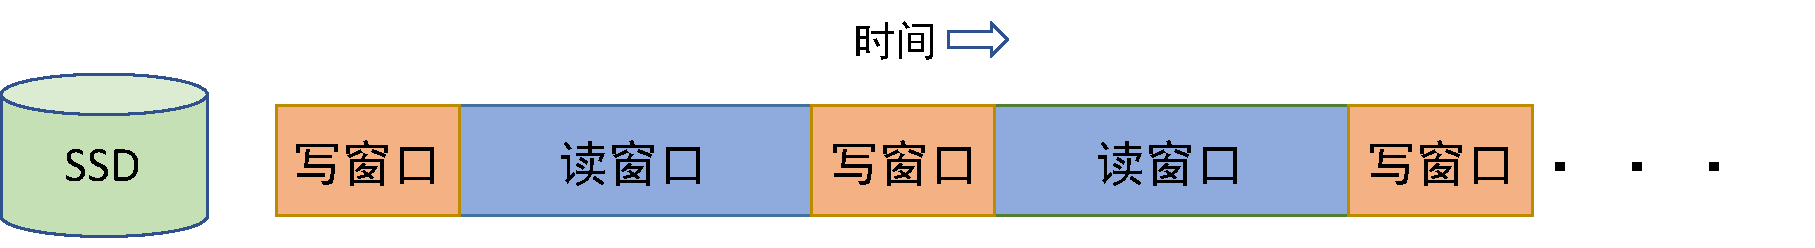
\includegraphics[width=0.8\textwidth]{thesis-iso-wr.pdf}
  \caption{
        分离的读写时间窗口在单块SSD上的工作流程。
        在读窗口中,所有写请求被缓存于缓冲区中,从而保证读请求的尾延迟;
        在写窗口中,之前被缓存的写请求被批量发送,充分利用SSD的写带宽。
      }
  \label{fig:design-iso-wr}
\end{figure}

\JF{图.b}描述了分离的读写时间窗口对SSD的读延迟分布的影响。
通过将写操作在写窗口中批量发送,所有可能出现异常读延迟的情况都被限制在了写窗口中。
通过避免在写窗口中发送读请求,租户可以在在读窗口中获得稳定的读延迟。

\subsection{读写窗口协调的冗余磁盘阵列}
\label{sec:design-array-composition}

尽管上一节提出的分离的读写窗口可以使读请求在读窗口中得到不受干扰的读延迟,但它不能在写窗口中接受读请求。
对于现代的在线事务处理服务来讲,对于存储服务的读访问往往处于其关键路径上。
因此,单块SSD的写窗口时间如果过长,会导致其读访问排队延迟过大,使得分离的读写窗口得不偿失。

遗憾的是,在实践中,写窗口的时间不能很短。
由\JF{图}可见,即使写窗口已经结束,下一个读窗口起始处的一些读请求仍会出现异常延迟。
这是由于写操作触发的垃圾回收、缓冲区刷新等SSD内部维护操作是异步进行的。
在写操作完成后,这些操作仍在进行,从而影响后续读操作的延迟。
因此,SSD上读写窗口的时间不能过短,否则过于频繁的窗口切换会影响大量读请求的延迟,从而大大影响总体的尾延迟。

针对这一问题,本研究提出使用\textit{具有冗余的SSD阵列}来掩盖SSD的写窗口。
由于具有冗余的SSD阵列(例如RAID~\cite{patterson1988case}或纠删码~\cite{huang2012erasure})具有从若干台SSD的故障中恢复的能力,所以可以将处于写窗口中的SSD视为“故障”。
通过协调各个SSD上的读写窗口,可以保证同时处于写窗口中的SSD数量不多于阵列的恢复能力。
当有面向处于写窗口中的SSD数据的读请求时,可以利用其它SSD中的数据恢复该SSD中的数据。
由于其它SSD均处于读窗口中,具有良好的访问延迟,因此对处于写窗口中SSD数据的恢复也具有良好的延迟。

\begin{figure}[h]
  \centering
  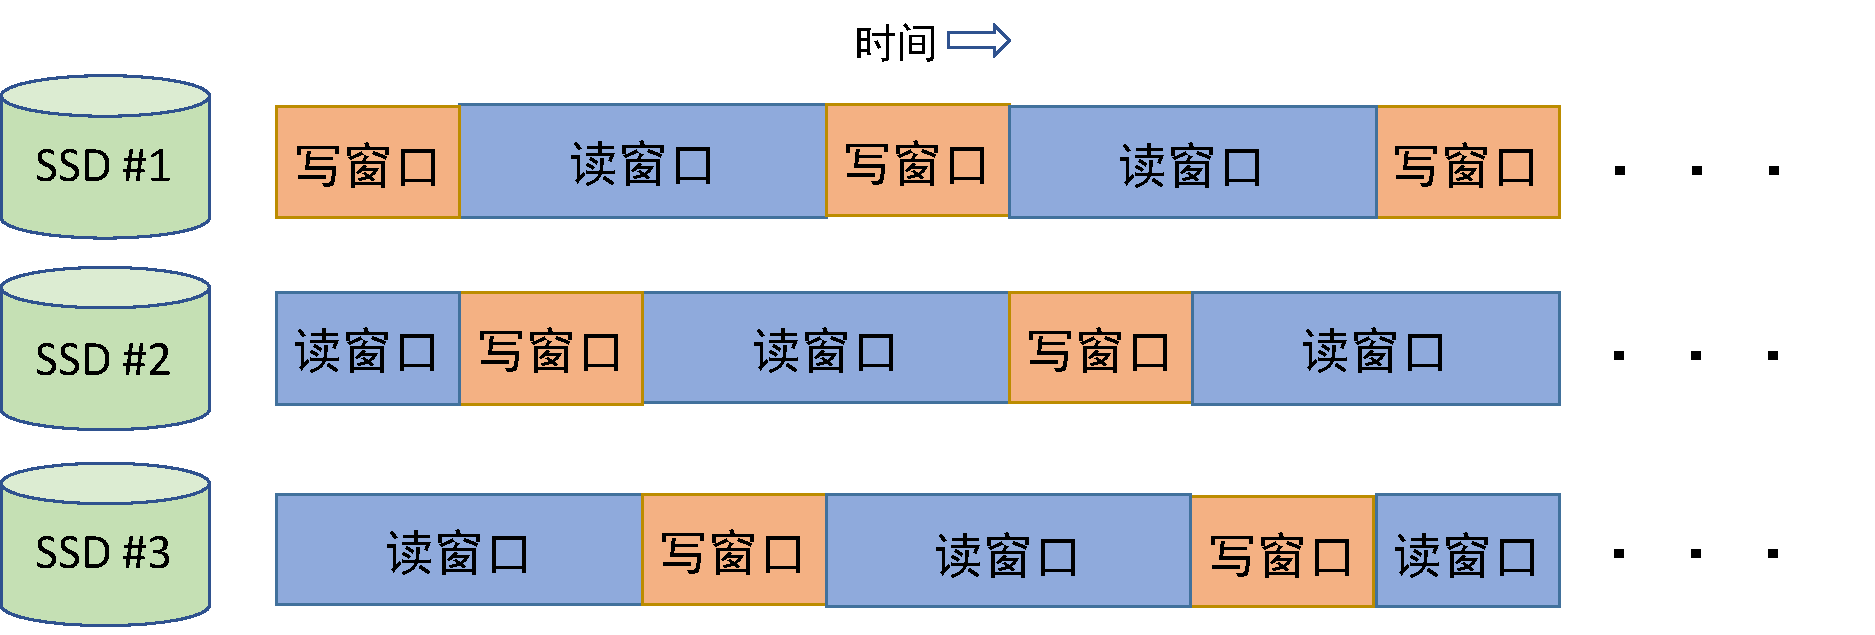
\includegraphics[width=0.8\textwidth]{thesis-ssd-array.pdf}
  \caption{
        用RAID-5组成读写窗口协调的冗余SSD阵列。
        通过协调各个SSD上的读写窗口,可以保证同时最多有一台SSD处于写窗口。
        由于RAID-5可以从一块磁盘的故障中恢复,所以所有数据总可以被以无干扰的读延迟访问。
      }
  \label{fig:design-ssd-array}
\end{figure}

例如,在\autoref{fig:design-ssd-array}中,利用3块SSD组成了一个RAID-5磁盘阵列。
通过协调三台SSD交替进入写窗口,该阵列保证任一时间都只有一台SSD不可读。
由于RAID-5具有从一块磁盘故障中恢复的能力,因此对所有数据的读都有较低的尾延迟。
比如当SSD \#1处于写窗口时,对其中数据的读,可以通过先读取SSD \#2和SSD \#3的相应数据,之后进行异或运算实现。

\section{满足SLA要求的数据分布算法}
\label{sec:design-allocation}

通过构建无读写干扰的SSD阵列,

\subsection{SLA曲线及其运算}
\label{sec:design-allocation-sla-arithmetic}

加法、减法。

\subsection{多租户数据分布算法}
\label{sec:design-allocation-algo}

\IncMargin{1em}
\begin{algorithm}[h]
  \SetAlgoLined
  \SetKwData{Suitable}{unitChoices}\SetKwData{SortedUnits}{sortedUnits}
  \SetKwData{Request}{request}\SetKwData{OpenUnits}{openUnits}\SetKwData{UnitTypes}{unitTypes}
  \SetKwData{U}{u}
  \SetKwData{UT}{ut}
  \SetKwData{BestType}{bestType}
  \SetKwData{BestCost}{bestCost}
  \SetKwData{CostForRequest}{costForRequest}
  \SetKwFunction{Filter}{Filter}
  \SetKwFunction{Fitness}{Fitness}
  \KwData{用户请求\Request,已启用的存储单元列表\OpenUnits,可选的存储单元类型\UnitTypes,均以$(C, S, T)$的形式表示,每个存储单元类型有开销$P$}
  \BlankLine

  \tcp{将\Request 中的数据块尽可能存入已开启的存储单元中}
  \Suitable$\leftarrow$ \Filter{\OpenUnits, \Request.T} \;% $\leftarrow$ \;% \Filter{$open\_units$, $request\.T$}\;
  将 \Suitable 按 \Fitness 函数排序 \;

  \ForEach{\Suitable 中的存储单元\U}{
    尽可能多地将\Request 中的数据块存放于\U 中 \;
    \lIf(\tcp*[h]{\Request 中所有的数据块都已分配完毕}){\Request $.C$ == 0}{
      \Return{}
    }
  }

  \tcp{需要启用新的存储单元,贪心地选择用最小开销容纳剩余的数据块}
  
  \BestCost $\leftarrow$ $+\infty$

  \ForEach{\UnitTypes 中的存储单元类型\UT}{
    \CostForRequest $\leftarrow$ 容纳\Request 所需的\UT 个数$\times$\UT .P \;
    \If{\CostForRequest $<$ \BestCost}{
      \BestType $\leftarrow$ \UT \;
    }
  }

  启用\BestType 类型存储单元来存放\Request 中的数据块 \;

  \caption{租户进入系统时的数据分布算法}
  \label{algo:tenant-allocation}
\end{algorithm}
\DecMargin{1em}
